\section{Drone Navigation}

\subsection{Functional Requirements}

	\begin{flushleft}
		\begin{itemize}
			\item [\textbf{R1:}] FMDS will \textbf{follow} the ranger

		  		\begin{itemize}
		  			\item  [\textbf{R1.1}] FMDS will allow the ranger to perform \textbf{initialisation} for the drone.
		  				\begin{itemize}
		  					\item [\textbf{R1.1.1}] FMDS will allow the ranger to set himself as the validated object.
		  					\item [\textbf{R1.1.2}] FMDS will allow the ranger to initialise his beacon. 
		  				\end{itemize}

		  			\item  [\textbf{R1.2}] FMDS will allow the ranger to specify a \textbf{flight pattern} for the drone
		  				\begin{itemize}
		  					\item [\textbf{R1.2.1}] FMDS will detect objects while on its flight path.
		  					\item [\textbf{R1.2.2}] FMDS will record live video while on its flight path.
						  \end{itemize}
			\end{itemize}
		\end{itemize}

		\begin{itemize}
			\item [\textbf{R2:}] FMDS will \textbf{patrol} the area around the ranger

				\begin{itemize}
					\item [\textbf{R2.1}] FMDS will patrol by flying in the designated \textbf{flight pattern} around the ranger.
					\item [\textbf{R2.2}] FMDS will perform \textbf{object detection}.
						\begin{itemize}
							\item [\textbf{R2.2.1}] FMDS will drop a pin of the object detected on the 2D map.
						\end{itemize}
					\item [\textbf{R2.3}] FMDS will \textbf{record} video footage during it's surveillance.
					\item [\textbf{R2.4}] FMDS will take \textbf{snapshots} of the reserve during it's surveillance.
						\begin{itemize}
							\item [\textbf{R2.4.1}] FMDS will build a 2D map of the reserve.
						\end{itemize}
				\end{itemize}
		\end{itemize}
	\end{flushleft}

\subsection{Use Case Diagram}
\begin{center}
	\begin{flushleft}
		\begin{figure}[h!]
			\centering
			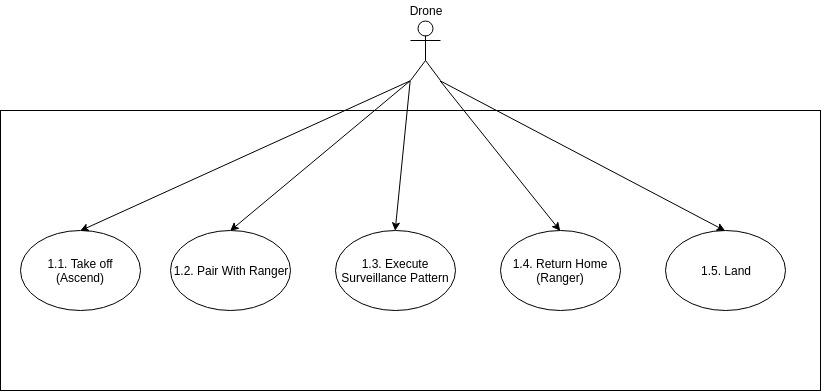
\includegraphics[scale=0.5]{./assets/images/navigation-ucd.jpg}
			\label{fig: object-recognition-ucd }
			\caption{Drone Navigation Use Case Diagram}
		\end{figure}

	\end{flushleft}
\end{center}
